\documentclass{article}
\usepackage[dvipsnames]{xcolor}
\usepackage{pgfplots}
\usepackage{adjustbox}
\usepackage{appendix}
\usepackage[T1]{fontenc}
\usepackage{lmodern}
\pgfplotsset{compat=1.15}
\newcount\recurdepth

\newcommand\storelabel[2]{\expandafter\xdef\csname label#1\endcsname{#2}}
\newcommand\getlabel[1]{\csname label#1\endcsname}
\newcommand{\absval}[1]{\ifnum#1<0 -\fi#1}

% if you need to pass options to natbib, use, e.g.:
%     \PassOptionsToPackage{numbers, compress}{natbib}
% before loading neurips_2019

% ready for submission
% \usepackage{neurips_2019}

% to compile a preprint version, e.g., for submission to arXiv, add add the
% [preprint] option:
%     \usepackage[preprint]{neurips_2019}

% to compile a camera-ready version, add the [final] option, e.g.:
%    \usepackage[final]{neurips_2019}

% to avoid loading the natbib package, add option nonatbib:
%     \usepackage[nonatbib]{neurips_2019}

\usepackage[utf8]{inputenc} % allow utf-8 input
\usepackage[T1]{fontenc}    % use 8-bit T1 fonts
\usepackage{hyperref}       % hyperlinks
\usepackage{url}            % simple URL typesetting
\usepackage{booktabs}       % professional-quality tables
\usepackage{amsfonts}       % blackboard math symbols
\usepackage{amsmath}
\usepackage{nicefrac}       % compact symbols for 1/2, etc.
\usepackage{microtype}      % microtypography
\usepackage{tikz}
\usetikzlibrary{arrows}
\usetikzlibrary{matrix}
\usetikzlibrary{positioning}
\usepackage{bnumexpr}
\usepackage{forloop}
\usepackage{xfp}

\title{Fractal Neural Networks as Ensembles of Continuous-Valued Cellular Automata: Pathfinding and Related Problems of Variable Scale}

% The \author macro works with any number of authors. There are two commands
% used to separate the names and addresses of multiple authors: \And and \AND.
%
% Using \And between authors leaves it to LaTeX to determine where to break the
% lines. Using \AND forces a line break at that point. So, if LaTeX puts 3 of 4
% authors names on the first line, and the last on the second line, try using
% \AND instead of \And before the third author name.

\author{%
  Sam Earle
    %\thanks{Use footnote for providing further information
%   about author (webpage, alternative address)---\emph{not} for acknowledging
%   funding agencies.} \\
%    \texttt{smearle93@gmail.com} \\
  % examples of more authors
  % \And
  % Coauthor \\
  % Affiliation \\
  % Address \\
  % \texttt{email} \\
  % \AND
  % Coauthor \\
  % Affiliation \\
  % Address \\
  % \texttt{email} \\
  % \And
  % Coauthor \\
  % Affiliation \\
  % Address \\
  % \texttt{email} \\
  % \And
  % Coauthor \\
  % Affiliation \\
  % Address \\
  % \texttt{email} \\
}

\begin{document}

%\tableofcontents
\newpage
\maketitle

\begin{abstract}
We suggest that any agent playing a game with variable map-size should learn a map-size-invariant gameplay policy. 
Inspired by recent Reinforcement Learning environments with scalable maps---and scalable 2D observation and action spaces along with them---we consider a simple, scalable, pathfinding problem. 
Curious as to how trainable Neural Networks might come to solve such problems in a truly map-size-invariant manner, we outline an implementation of a path-finding Cellular Automoton as a recursive, convolutional NN, albeit with an atypical, periodic activation function.
We note the structural equivalence between this manual implementation of a continuous-valued CA, and a single column of a Fractal Neural Network with weight-sharing.
We consider whether FNNs might be able learn policies similar to the one encoded in our Neural CA.  
To guarantee agents access to coarse map-features, we propose an alternate, explicitly dimensionality-reducing FNN model.
\end{abstract}

\section{Introduction}

We propose a new desideratum for strategy-game-playing and related Reinforcement Learning agents.
We expect any agent whose observation and action-spaces can be represented as $n-$dimensional grids to be able to transfer its skills to larger $n-$dimensional grids, insofar as they represent the same game at a different scale.
Human Go players, for example, sometimes practice on smaller boards to hone elements of strategy that are applicable to games on larger boards.
In popular strategy games like Civilization, various map-sizes are offered (and the player usually advised to start small).
If an agent can be said to have developed a behavioural policy that properly represents the game-elements and the relations between them, then this policy should be effective at multiple scales.


% We restrict ourselves to speaking of how the agent's behaviour accounts for its environment---though we'd rather say that the right conceptual model of the game will allow an agent to scale its play.
%In many RL agents, however, no model of the environment, nor symbols that represent categories within it, can be reliably located.
%Recent work, however, has had success training agents that leverage auxiliary linguistic models corresponding to its environment, in order to guide its behaviour within it \cite{hu2019hierarchical}.
%Other work has shown that both sentences and images can be parsed by recursive neural networks which are trained to identify the recursive structure of their inputs \cite{socher2011parsing}.
%In this work we emphasize the recursive structure of certain RL environments, and subsequently make a case for agents that use recursive processing in order to act within them.
%By extension, we argue, these agents are well-suited to performing tasks at variable scales.

%Replace path-planning with spanning trees
Consider a simple example, in which an agent receives as its input a full view of a maze, represented as a connected subset of a 2D grid, and must colour the shortest path between source and target nodes in the maze, edge by edge.
A standard path-finding algorithm could solve this task regardless of maze size, but the neural network models used to encode the behavioural policy of the RL agents commonly applied to arcade and strategy games are not capable of scaling up their policy to act on input sizes larger than were trained upon without training of additional parameters. 
% Power Puzzle is just pathfinding in the right order

We show, with a fixed and hand-weighted neural network which implements a continuous-valued Cellular Automoton---that sufficiently deep, recursive networks can solve a time-sensitive minimal spanning tree task at multiple scales. % Do we RLY show this, experimentally, though?
We are not necessarily interested in path-finding specifically, but take it as a good minimal example of a task that requires an agent to leverage spatial relationships between features of arbitrarily large maps.
By implementing a CA that solves this task deterministically as a recursive NN, we intend to show that recursive NN architectures are a natural fit for agents trained to play strategy games at various board sizes. 

In concurrent work (\ref{app:gymcity}), we introduce 3 RL environments that support scaling of the gameboard: a tile-by-tile board-filling task in Conway's Game of Life---with a randomly initialized array of cells---(\ref{app:GoL}); a time-sensitive, randomized minimal-spanning-tree problem in SimCity1---framed in terms of power deliver---(\ref{app:PP}); and a general population-maximization problem in SC---in which the agent can build any zone/structure/land-feature---(\ref{app:SC}).
In each, the agent has the full multi-channel 2D gameboard as its observation space, and the same 2D board with build-specific channels as its action space.
In SimCity, it is natural to expect optimal ``city planners'' to be near-optimal ``Regional Planners;'' they both deal with the same problems of road- and power-network layout, and the spatial distribution of different zone types---relations that play out according to the same local rules at every map size (though they may contribute to different global dynamics at different scales, as is the case for extra-municipal demand for zone-by-type, where demand can fluctuate more intensely on larger maps with larger populations).

We use recursive neural networks to do $0$-shot transfer to larger gameboards in our RL environments, with varying success (Figures \ref{fig:big_ded.jpeg} and \ref{fig:GoL_builds}).
In particular, scaling up the spanning-tree problem---by design---demands that the agent's network increase in depth, because the problem cannot be solved optimally without sufficiently large receptive fields.
This motivates the use of NNs generated by a repeated `fractal' expansion rule, and sharing a single set of weights; because these networks---by re-application of the expansion rule---can increase in depth and receptive-field size, in a natural and structurally coherent manner. 

In pursuit of similarly transferable skills, Compositional Pattern Producing Networks have been used to generate indirect encodings of NNs---which scale with observation and action-space size---to do $0$-shot transfer to octopus arms with more segments, in an octopus-arm control task \cite{woolley2010evolving}.
Similarly, NerveNet \cite{wang2018nervenet} uses Graph NNs to to $0$-shot transfer to 3D agents with more complex bodies (where limb connectivity is represented by a graph).
It would be interesting to consider whether or how a CPPN could produce recursive, convolutional networks like those presented here.
%It is also of note that the adjacency relationships on our 2D board form a 2D lattice---potential input to a Graph NN.

\section{Scalable, parallelized pathfinding}



Cellular Automata have been used extensively for pathfinding \cite{singhal2014review, rosenstiehl1972intelligent}.
%\cite{rosenstiehl1972intelligent} uses CA to implement pathfinding and spanning-tree algorithms over finite graphs of cells. % details ?
Slime mould has been used to solve mazes \cite{adamatzky2012slime} and plan road networks between sources and sinks \cite{adamatzky2010road}, the starved mould spreading out from its starting position toward nutrient sources. Its behaviour was subsequently modeled using CA \cite{tsompanas2016cellular}. % how?
% Not exhaustive, but context, and points of reference to stabilize the rest of the paper

In \cite{behring2001algorithm}, CA have likewise been used for pathfinding, guiding a token through a 2D grid littered with obstacles toward targets, by moving in one of the four cardinal directions at each step.
They use a CA to calculate the Manhattan distance, by 'flooding' the map with an activation that spreads out from the goal to path-adjacent tiles. 
With each tick, newly-activated tiles are given incrementally higher values than at the step previous, in order to track the time in which they were reached by the flood.

Our implementation was initially designed in order to generate a minimal-spanning tree, in order to solve an electricity-delivery problem over a sparse urban grid, and can thus have multiple sources (nodes in the spanning tree) and targets (nodes not in the spanning tree) at any particular step.
In order to facilitate its implementation as an FNN, our CA simultaneously floods outward from sources and targets, and finds an ordering by manhattan distance of all tiles that are in the middle of some path from a source to a target.
%Note that a pathfinding problem relying on local actions is a minimal-spanning tree generation problem (demanding a tree with only 2 nodes), wherein each newly-added edge must must belong to the existing tree.







%Our implementation, on the other hand, would repeatedly build edges in the middle of the shortest path between the existing tree, and any disconnected node (or agent-placed edge),





\subsection{Spanning Trees with Recursive Neural Networks}

In appendix \ref{app:CA}, we define a CA capable of solving minimal-spanning-tree problems at multiple scales. 
We intentionally define the CA using more channels than necessary, to make it functionally identical to its neural implementation.

Our neural network is convolutional, recursive and and as deep as necessary for the CA it implements to complete its computation. 
It consists of one set of convolutional weights applied repeatedly to an activation state.
This recursive body is book-ended by $1\times 1$-kernel convolutional layers to map the agent's hidden activation to and from the output and input spaces, respectively.
On the way in, existing channels of the board are copied to a few channels of activation space, while the rest is left empty.


% Verify all marks are in fact possible computation-spots in our implementation!!

\begin{figure}
\pgfplotsset{
possible/.style={dashed, thick, samples=100, color =PineGreen}}
\pgfplotsset{width=13cm, height=4cm}
\begin{tikzpicture}[every mark/.append style={mark size=1.5pt}]
    \pgfmathsetlengthmacro\MajorTickLength{
      \pgfkeysvalueof{/pgfplots/major tick length} * 2
		}
  \begin{axis}[domain  = -21:35,
							 axis x line = center,
							 axis y line = center,
               samples = 100,
               xmin    = -20,
               xmax    = 36,
							 ymin    = -.5,
							 ymax    = 1.5,
							 xtick={},
							 ytick={1},
							 xtick   = {-20, -16, -12, -8, -4, 0, 1, 6, 12, 18, 23, 26, 29, 32},
               xlabel  = {$a$},
							 ylabel  = {$g(a)$},
               set layers,
							 every axis plot/.append style={blue},
							 x label style={
							 anchor=west,},
							 y label style={
							 anchor=south,
							 },
							 major tick length = \MajorTickLength,
							 every tick/.style={
							 black,
						 semithick,},
							 minor tick num = 4,
							 legend cell align=left,
							 legend style={fill=white, fill opacity=0.6, text opacity=1, draw=none, font=\footnotesize, at={(-.05,1.1,0)}, anchor=north west},
							 grid = both,
               ]
							\addplot[domain= -23:0, possible] {0};
							\addplot[domain= 0:1, possible, forget plot] {x};
				\addplot[possible, domain= 1:5, forget plot] coordinates{
			(1, 1)
			(2, 1)
			(3, 1)
			(4, 1)
			(5, 1)
			(6, 0) (7, 1) (11, 1) 
			(12, 0) (13, 1) (17, 1) 
			(18, 0) (19, 1)
			(20, 1)
			(35, 1)
	};
							 \addplot[samples=100, only marks, domain=-20:0, mark=*, opacity=0.5] coordinates{
							 (-20, 0) 
						   (-16, 0) 
							 (-15, 0) 
						   (-12, 0) (-11, 0) 
						(-10, 0) 
					(-8, 0) (-7, 0) (-6, 0) (-5, 0) 
				(-4, 0) (-3, 0) (-2, 0) (-1, 0) (0, 0)
			(20,1)
			(23, 1)
			(24, 1)
			(26, 1)
			(27, 1) (28, 1)
			(29, 1)
			(30, 1) (31, 1) 
			(32, 1)
			(33, 1) (34, 1) (35, 1) (36, 1)

			(1, 1)
			(2, 1)
			(3, 1)
			(4, 1)
			};

	\addplot[only marks, color=red, opacity=0.5, samples=100, domain= 1:5, mark=*] coordinates{
		(-6,0) (-5, 0) (-4, 0) (-3,-0) (-2, 0) (-1,0)
		(0,0) 
			(1, 1)
			(2, 1)
			(3, 1)
			(4, 1)
			(6, 0) (7, 1) (8, 1) (9, 1) 
			(12, 0) (13, 1) (14, 1)
			(18, 0) (19, 1)
			(1/2, 1/2)
					(3/4, 3/4)
					(5/8, 5/8)
					(11/16, 11/16)
					(21/32, 21/32)
					(43/64, 43/63)
	};
				\addplot[only marks, samples=100, domain= 0:1, color=green!50!gray, opacity=0.5] coordinates{
					(1, 1)
					(1/2, 1/2)
					(1/4, 1/4)
					(1/8, 1/8)
					(1/16, 1/16)
					(1/32, 1/32)
					(1/64, 1/64)
					(1/128, 1/128)
					(1/256, 1/256)
					(1/512, 1/512)

	};

	\addlegendentry{possible nonlinearity $g(a)$}
\addlegendentry{activations in $R$ and $S$}
\addlegendentry{'' in channel $U$}
\addlegendentry{'' in $W$}
\end{axis}
\end{tikzpicture}

\caption{A sufficient activation function for our Neural CA, which performs computations only at the specified points.}
\label{fig:activation}
\end{figure}

We use the same nonlinear activation function ($g(a)$ in Figure \ref{fig:activation}) at each layer. 
$g(a)$ can be seen as the combination of a hard tanh function with a periodic one.
In general, some weights $b_{A}$ feed activation from a $3\times 3$ spatial patch, to its central node---and from channel $A$ to channel $B$---of subsequent activation-maps. The values of particular weights will be given by: 

\begin{align*}
	b_{A} = \begin{bmatrix}
		b_{-1, 1} & b_{0, 1} & b_{1, 1} \\
		b_{-1, 0} & b_{0, 0} & b_{1, 0} \\
		b_{-1, -1} & b_{0, -1} & b_{1, -1}\\
	\end{bmatrix}
\end{align*}
, 	where $m_{j, k}$ is the value of the weight leading from the node that is $j$ and $k$ cells over from the central node. The bias at neurons in $B$ is denoted by $b_\text{BIAS}$ and left equal to $0$ unless otherwise specified.


First, let us define the following constant convolutional weights:
\begin{align*}
	m_{\text{vn}} = \begin{bmatrix}
		0 & 1 & 0 \\
		1 & 1 & 1 \\
		0 & 1 & 0 \\
	\end{bmatrix} &&
	m_\text{c} = \begin{bmatrix}
		0 & 0 & 0 \\
		0 & 1 & 0 \\
		0 & 0 & 0 \\
\end{bmatrix}
\end{align*}
. Then we characterize the channels $R$ and $S$ by their convolutional weights:
\begin{align*}
&r_{R} = s_{S} = m_\text{vn} + 31(m_\text{c})&&
	r_{S} = s_{R} = -3 (m_\text{vn}) &&
	r_{O} = s_{O} = -4 (m_\text{c}) && \\
	%&r_{R'} = s_{S'} = 32(m_\text{c}) Then you'd need to draw way more points on nonlinearity plot 
\end{align*}
, where the first rules allow the permanent spread of activation floods on their respective channels, the second ensures that these floods come to a halt upon meeting in space, and the third prevents floods from entering tiles occupied by an obstacle (where $O$ is the fixed, binary obstacle channel). Both rules are affected by the hardtanh structure of the nonlinearity, using appropriately sized weights to `skip' the periodic stretch as necessary.

The gate channel $U$ is given by 
\begin{align*}
	&	u_R = 6(m_\text{vn}) &&u_\text{BIAS}=-6 &&u_U = -1/2(m_\text{c}) \\
	& u_S = m_\text{vn}
\end{align*}
. Using the periodic structure of the nonlinearity, when both floods enter the VN patch, an activation of $1$ will arise (after the bias).
After this cell is activated, it oscillates between $1/2$ and $3/4$, converging to $2/3$, thus remaining semi-active to prevent a repeat activation of $1$. 

For the binary out-gate:
\begin{align*}
	& v_U = 4 && v_\text{BIAS} = -3
\end{align*}
, taking advantage of the fact that $U$ has all $u_i \not\in (\frac{3}{4}, 1]$

Our timekeeper $W$ has only to start `counting' when the gate fires:

\begin{align*}
	& w_V = m_\text{c} && w_W = 1/2(m_\text{c})
\end{align*}
. Finally, an output channel stores the earliest collision-site as a maximum value:
\begin{align*}
	o_W = -1(m_\text{c}) && o_{\text{BIAS}} = 1
\end{align*}
. After a $1\times 1$ embedding copying only this layer, its highest-valued tile is selected as the site of an edge-build.



\section{Considerations for Learning Agents}

The kind of activation function required by the above neural implementation is more complex than the simple ReLU activation used in our RL experiments and common in convolutional NN's.
In particular, the periodic stretch's non-monotonicity could make it impossible to train weights via backpropogation \cite{parascandolo2017taming}.
We might still, however, entertain the possibility that a neuro-evolutionary algorithm could be able to replace the need for backpropogation---either by evolving weight-values (as does NEAT \cite{stanley2002evolving}) or ignoring them entirely \cite{gaier2019weight}.

In a similar vein, \cite{hagg2017evolving} extends NEAT with a mutation that switches one for another of a predetermined list of activation functions.
But NEAT could also be applied to evolve a Compositional Pattern-Producing Network \cite{stanley2009hypercube} (with $1$ input and output dimension)---which, notably, are well-suited to generating periodic functions---to encode the activation function.

Or, more simply, we could hope that---by taking advantage of more channels to the hidden activation-state, and/or more densely populating weight-matrices than in our sparse manual implementation---the trained network could manage to approximate the behaviour of our CA by other means, in spite of a simpler non-linearity.

It is interesting to note that the activation function is only specified for a particular set of points on an interval of the real number line.
Our implementation computes certain discrete values at a fixed number of points, along with certain convergent sequences.
We could continue to implement additional CA rules in new channels, by following the existing strategy, and scaling and transforming input to the nonlinearity as necessary, so that it could co-occur with the existing rules, with computations taking place on a different subset of the activation function.

We should note that the use of convergent series may pose practical difficulties as the floating-point accuracy needed to differentiate certain activations grows exponentially with the number of ticks. Scaling activations and adding appropriate curvature to the activation function might help in combatting this issue.

Future work should examine if it is possible to create a mapping from any one of some subset of CAs, to a single set of convolutional weights (interpreted as the shared weights of a single, sufficiently-deep, recursive neural ``column'') and an accompanying activation function.
If it is, we could gain a new level of abstraction in discussing the behaviour of trained or evolved recursive neural networks, by exploiting the inverse mapping to extract CAs from the network; or, we could use the language of CAs as a new and automatic means for providing strong built-in priors to trainable NNs. 

Even our manually-implemented CA could be run in parallel with a trainable model---a nontrainable extension of it, over which backpropogation does not occur---sharing its activations with the agent, and vice verse, with each concurrent tick.
Such an approach would be similar in spirit to RL approaches that train agents to leverage auxiliary language models relating to the environment \cite{hu2019hierarchical}, though CA `languages' are conceptually much lower-level than conventional ones.

%If nothing else, our implementation gives a specific use-case for (truncated) periodic activations functions, namely, to discern the co-occurence of activations in two distinct channels within the same patch of activation space.
%Our nonlinearity, for example, outputs $2$ only when `source' and `target' flows enter the same neighbourhood.


%Recent work has shown that networks capable of performing simple RL control tasks can be evolved using the NEAT neuro-evolutionary algorithm, assigning a single random number to all weights in the network.
%If we can


\newcount\nodewidth
\nodewidth=48
\newcount\ncols
	\tikzset{equal/.style={draw, dotted, very thick}}
	\tikzset{joinlayer/.style={draw, dashed, very thick}}
	\tikzset{down/.style={draw, ->, BrickRed ,very thick}}
	\tikzset{up/.style={draw, ->, OliveGreen, very thick}}
	\tikzset{conv/.style={draw, ->, very thick}}
	\tikzset{convlabel/.style={anchor=west,inner sep=5, color=black}}
	\tikzset{hidden/.style={rectangle, draw, minimum width=\nodewidth, align=center, fill=gray, 
	fill opacity=0.1}}
	\tikzset{legendtext/.style={anchor=west,inner sep=10, color=black, text height=0.1mm}}
\begin{figure*}
\begin{tikzpicture}[scale=1]


	\matrix [at={(1.3,-1.8)},  minimum height=1, anchor=north west, font=\footnotesize] {
	\draw[conv] (0,0) -- node[legendtext] {Convolution $f$} (0.6,0);& \\
	\draw[down] (0,0) -- node[legendtext] {Strided Convolution $d$} (0.6,0);\\
	\draw[up] (0,0) -- node[legendtext] {Transposed Convolution $u$} (0.6,0);\\
		\node [hidden, label=right: ($32\times32$) Activation Map] {};\\
		\node [hidden, minimum width=\nodewidth/2, fill opacity=0.4, align=center, label=right: ($16\times16$) ''] at (12pt, 0){};  \\
		\node [hidden, minimum width=\nodewidth/4, fill opacity=1,label=right:($8\times 8$) ''] at (18pt, 0){}; \\
	\draw[joinlayer] (0,0) -- node[legendtext] {Join Operation} (0.6,0);\\
	\draw[equal] (0,0) -- node[legendtext] {Equality} (0.6,0);\\
};

\def\fracnet#1#2#3#4{
	\newcount\yscale
	\yscale=4
  \edef\col{\number\numexpr#1\relax}%a+b
  \edef\dep{\number\numexpr#2}%a+b
	\edef\ypos{\number\numexpr#3\relax}
  \edef\incol{\number\numexpr\ncols-\col\relax}%a+b
  \edef\subcolh{\bnumexpr2^(\col)\relax}
	\edef\maxdepth{\bnumexpr2^(\ncols-1)\relax}
 	\edef\coldepth{\bnumexpr\number2^(\ncols-\number\col)\relax}
	\edef\yposI{\number\numexpr\ypos+\bnethe\subcolh\relax}
	\edef\yposO{\number\numexpr\ypos-\bnethe\subcolh\relax}
%\node[draw=none] at (\number\col*2 + 0.75, \ypos/\yscale) {\col, $\ypos$, \bnethe\subcolh, \bnethe\coldepth, \dep};
	\edef\colname{\number\numexpr\col-1\relax}
%\storelabel{\col-\yposI}{\aI}
	\node[hidden, name=#4\col\yposO] at (\number\col*2, \yposO/\yscale) {};
 \edef\dblmaxdepth{\bnumexpr\maxdepth*2\relax}
 \edef\firstdep{\bnumexpr\dblmaxdepth-\yposI\relax}
 \ifnum\bnethe\firstdep=0\relax
	 \node[hidden, name=#4\col\yposI] at (\number\col*2, \yposI/\yscale) {};
	\fi
	\draw[conv] (#4\col\yposI) -- node[convlabel] {$f_{\colname,\dep}$} (#4\col\yposO);
\ifnum\col>1\relax
	\begingroup
	\edef\col{\number\numexpr\number\col-1\relax}%a+b
	\edef\yposA{\number\numexpr\ypos+(\bnethe\subcolh/2)\relax}
	\edef\yposB{\number\numexpr\ypos-(\bnethe\subcolh/2)\relax}
	\edef\dep{\number\numexpr\dep*2\relax}
	\edef\depA{\number\numexpr\dep\relax}
	\edef\depB{\number\numexpr\dep+1\relax}
	\fracnet{\number\col}{\depA}{\number\yposA}{#4}
	\fracnet{\number\col}{\depB}{\number\yposB}{#4}
	\endgroup
\fi
\ifnum\col>1\relax
	\edef\nextcol{\number\numexpr\col-1\relax}
	\draw[joinlayer] (#4\col\yposO) edge (#4\nextcol\yposO);
	\ifnum\dep=0\relax
		\draw[equal] (#4\col\yposI) edge (#4\nextcol\yposI);
	\fi
\fi
}

\def\FracNet#1#2{
	\ncols=#1
	\fracnet{#1}{0}{0}{#2}
}

\node[hidden, draw=none, fill opacity=0, text opacity =1, font=\large] at (2,1.3) {$F^1$};
\FracNet{1}{A}
\tikzset{hidden/.append style={xshift=75, yshift=-14}}
\node[hidden, draw=none, fill opacity=0, text opacity =1, font=\large, yshift=14] at (3,1.3) {$F^2$};
\FracNet{2}{B}
\tikzset{hidden/.append style={xshift=125, yshift=-28}}
\node[hidden, draw=none, fill opacity=0, text opacity =1, font=\large, yshift=42] at (4,1.3) {$F^3$};
\FracNet{3}{B}
\tikzset{hidden/.append style={xshift=-125}}
\tikzset{hidden/.append style={yshift=-165}}

\def\fracnet#1#2#3#4{
	\newcount\yscale
	\yscale=3
  \edef\col{\number\numexpr#1\relax}%a+b
  \edef\dep{\number\numexpr#2}%a+b
	\edef\ypos{\number\numexpr#3\relax}
  \edef\incol{\number\numexpr\ncols-\col\relax}%a+b
  \edef\subcolh{\bnumexpr2^(\col)\relax}
	\edef\maxdepth{\bnumexpr2^(\ncols-1)\relax}
 	\edef\coldepth{\bnumexpr\number2^(\ncols-\number\col)\relax}
	\edef\yposI{\number\numexpr\ypos+\bnethe\subcolh\relax}
	\edef\yposO{\number\numexpr\ypos-\bnethe\subcolh\relax}
	\edef\nextcol{\number\numexpr\col-1\relax}
	\edef\lastcol{\number\numexpr\col+1\relax}
%\node[draw=none] at (\number\col*2 + 0.75, \ypos/\yscale) {\col, $\ypos$, \bnethe\subcolh, \bnethe\coldepth, \dep};
	\edef\colname{\number\numexpr\col-1\relax}
%\node[hidden, draw=none] at (\number\col*2 + 0.75, \ypos/\yscale) {$f_{\colname,\dep}$};
%\storelabel{\col-\yposI}{\aI}
	\node[hidden, draw,rectangle, label, name=#4\col\yposO] at (\number\col*2, \yposO/\yscale) {};
 \edef\dblmaxdepth{\bnumexpr\maxdepth*2\relax}
 \edef\firstdep{\bnumexpr\dblmaxdepth-\yposI\relax}
 \ifnum\bnethe\firstdep=0\relax
 \node[hidden, draw,rectangle,label, name=#4\col\yposI] at (\number\col*2, \yposI/\yscale) {};
	\fi
	\ifnum\col>1\relax
		\edef\dblcol{\bnumexpr(\col-1)\relax}
		\foreach \n in {1,...,\bnethe\dblcol}{
				\edef\uname{\number\numexpr\col-1-\n\relax}
				\edef\sqzstep{\bnumexpr\n-\col + 1\relax}
				\edef\skpwidth{\bnumexpr\nodewidth/(2*\n)\relax}
	%			\edef\skpos{\bnumexpr(\n)\relax}
				\edef\skpB{\bnumexpr((\col)*2-1)*\yscale\relax}
				\edef\skpA{\bnumexpr\n*2*\subcolh+\yposO*\skpB/\yscale\relax}				
				\node[hidden, fill opacity=0.1 + 0.3*\n*\n, rectangle, minimum width =\bnethe\skpwidth, name=u\col\dep\n] 
					at (\col*2, \bnethe\skpA/\bnethe\skpB) {};
				\edef\skpA{\bnumexpr-\n*2*\subcolh+\yposI*\skpB/\yscale\relax}		
				\node[hidden, fill opacity=0.1 + 0.3*\n*\n,rectangle, minimum width =\bnethe\skpwidth,name=d\col\dep\n] 
					at (\col*2, \bnethe\skpA/\bnethe\skpB) {};
				\ifnum \n=1
				 \draw[down] (#4\col\yposI)  -- node[convlabel] {$d_{\colname,\dep,\n}$} (d\col\dep\n);
				 \draw[up] (u\col\dep\n) -- node[convlabel] {$u_{\colname,\dep,\uname}$}  (#4\col\yposO);
				\else
					\edef\lastn{\number\numexpr\n-1\relax}
				  \draw[up] (u\col\dep\n) -- node[convlabel] {$u_{\colname,\dep,\uname}$} (u\col\dep\lastn);
					\draw[down] (d\col\dep\lastn) -- node[convlabel] {$d_{\colname,\dep,\n}$} (d\col\dep\n);
				\fi
				\edef\islastn{\bnumexpr\col-\n-1\relax}
				\ifnum\bnethe\islastn=0:
				%\draw[->] (d\col\dep\n) edge (u\col\dep\n);
					\draw[conv] (d\col\dep\n) -- node[convlabel] {$f_{\colname,\dep}$} (u\col\dep\n);
				\fi
	}
	\else
 \draw[conv] (#4\col\yposI) -- node[convlabel] {$f_{\colname,\dep}$} (#4\col\yposO);
	\fi
\ifnum\col>1\relax
	\begingroup
	\edef\col{\number\numexpr\number\col-1\relax}%a+b
	\edef\yposA{\number\numexpr\ypos+(\bnethe\subcolh/2)\relax}
	\edef\yposB{\number\numexpr\ypos-(\bnethe\subcolh/2)\relax}
	\edef\dep{\number\numexpr\dep*2\relax}
	\edef\depA{\number\numexpr\dep\relax}
	\edef\depB{\number\numexpr\dep+1\relax}
	\fracnet{\number\col}{\depA}{\number\yposA}{#4}
	\fracnet{\number\col}{\depB}{\number\yposB}{#4}
	\endgroup
\fi
\ifnum\col>1\relax
	\draw[joinlayer] (#4\col\yposO) edge (#4\nextcol\yposO);
	\ifnum\dep=0\relax
		\draw[equal] (#4\col\yposI) edge (#4\nextcol\yposI);
	\fi
\fi
}

\def\FracNet#1#2{
	\ncols=#1
	\fracnet{#1}{0}{0}{#2}
}

\tikzset{hidden/.append style={yshift=-38}}
\FracNet{2}{B}
\tikzset{hidden/.append style={xshift=125,yshift=38}}
\FracNet{3}{B}


\end{tikzpicture}
\caption{Fractal Neural Networks after the first three applications of the expansion rule for a regular FNN (above) and for a dimensionality-reducing FNN (below). With intra-column weight-sharing, then fixing only $j$ (the column index), all $f_{j,k,l}$, $d_{j,k,l}$ and $u_{j,k,l}$ share weights amongst themselves. With inter-column weight-sharing, there is one set of weights $f, d, u$, for each.}
\label{fig:frac}
\end{figure*}
\section{Fractal Neural Networks}


Fractal Neural Networks \cite{larsson2016fractalnet} were introduced to simplify ResNet's \cite{he2016deep} residual structure. 
With respect to the overall structure of standard ResNet, residual blocks are replaced by fractal blocks, though dimension-reducing blocks remain unchanged.
Fractal blocks result from a repeated expansion rule, which takes an existing network, copies it, and joins the copies to create a larger (twice as deep) network.
The nature of the expansion rule ensures that shallower paths run through the network at various scales, providing the same benefits as residuals, but with a more succinct structure.
In our concurrent work, we experiment with weight-sharing in FNNs, noting that with weight-sharing, the networks can be conceived of as ensembles of continuous-valued CA (\ref{app:nets}).

In a step toward likewise replacing the usual, max-pooling, down-/up-scaling blocks in Deep CNNs, we consider a new rule for fractal expansion that incorporates strided (downscaling) and transposed (upscaling) convolutions (Figure \ref{fig:frac}).
This allows for the agent to naturally adjust the amount of dimensionality-reduction performed dependent upon map size in an organic way.
In this rule, instead of using just a single convolution as a new skip connection, a single convolution is sandwhiched between pairs of down- and up-scaling convolutions---as many as the columns's index, and no more than possible for a given map-size.
FNNs generated by this new expansion rule have shown comparable performance to standard FNNs in preliminary experiments in our scalable RL environments.

%We are motivated in particular to remove max-pooling layers from our RL models by the structure of our city-planning task, where spatial information remains crucial at multiple scales.
%Additionally, since our agents should be able to perform at multiple scales, forcing our agent to deal with compressed representation of the map is desirable from a practical perspective; rather than iterating a few times over a very large state-space, it may be more effective in certain scenarios to shrink this state space before computing on it further.

By considering these dimensionality-reducing FNNs as ensembles of subnetworks with student-teacher dynamics---as in the original paper---we see that networks with lower-dimensional state-spaces can learn from networks with higher-dimensional states, allowing us to scale to compute demands during inference by extracting subnetworks of varying complexity.  

In neuroscience, Recurrent Fractal Neural Networks have been used to model the exchange of local and global information in visual input \cite{bieberich2002recurrent}. 
The interplay between coarse and fine-grained visual features is facilitated by a columnar fractal network structure which ensures the presence of short paths between neurons at various depths in the visual cortex. 
Our dimensionality-reducing columns make this interplay explicit, necessarily producing coarse representations---accounting for the possibility that deep columns of FNNs with fixed-dimension activation spaces learn fine-grained/localized features, their depth allowing global considerations without necessarily blurring local information; as is the case when deep, recursive neural networks \cite{kim2016deeply} with residuals \cite{tai2017image} are trained to perform image super-resolution.

%In considering the connectivity of a road network, and creating a spatially-compressed representation thereof, an agent might do well to know whether a connected stretch of road traverses a large of patch of land from one end to the other, but might be less so, if all it encodes is that there is some road, somewhere, within this larger patch. 
% ISN't this example moot, because local processing could simply store this information on reserved channels at every tile for max-pooling to later retrieve?
	% Only if you have coordinate information in the activation-state could you hope to keep it specific to regional patches. Local computation reports on region for each cell, then strided layer responds to this global trend at a higher level.




% As we expand the squeeze model toward infinity, additional columns can be considered as a network which, with minimal parameters, considers the entire input, to affect action anywhere on the board, potentially honing in on certain subpatches of input and output space, and, rather than simply attempting to encode a generic, copmpressed representation of the board, produce a focused reading of a particular 




\section{Future Work and Conclusion}

The `Squeeze' FNN has columns whose structure evoke the notion of `strided' and `transposed' CA.
In such a CA, rules could be applied to patches of the board in stride, in order to compress it; or map smaller patches to larger ones in order to expand it. 
If such a CA is randomly initialized on an infinite plane, it can tick forever while scaling dimension in either direction. 

A countercurrent of research has suggested that increasing the width of deep NNs is a viable alternative to increasing their depth \cite{zagoruyko2016wide}.
A third expansion rule can be conceived, which copies the network and runs the copies in parallel; it sandwiches the original between a new pair of down-/up-scaling layers, with the copy acting as a skip connection between activations on either side of this new pair.
After repetition, it results in a structure where skip connections traverse chains of downscaling-followed-by upscaling at various depths---between various pairs of activations of equal resolution (rather than just at the extremities, between full-size activations)---allowing the network to overlay coarse with fine-grained features at multiple scales.

We expect that requiring agents to perform at arbitrary map-sizes will narrow the task of learning generalizable representations of game elements.
It is easy to imagine how most canonical RL strategy or arcade environments might scale to larger map sizes, in theory if not already in practice. 
With slight alteration of certain existing environments (strategy and board games in particular, in addition to the newly-introduced simulation-games discussed here), we could measure the map-size-invariance of policies learned by RL agents across a wide variety of tasks.

But to train agents capable of such $0$-shot scaling, we need a scale-invariant, indirect encoding of the network.
We thus propose the use of FNNs with weight sharing to encode sets of weights that can be combined (via fractal expansion) to form NN architectures of variable complexity.
This agent-side complexity can then be scaled in tandem with map-size complexity, providing the agent with enough `compute time'---or large enough receptive fields---to properly consider the entire map at each step.

Continuous-valued Cellular Automata are presented as a possible explanatory framework for scalable FNNs of this sort, while out our Neural CA could provide a baseline in the minimal-spanning-tree task for NN-based RL agents. 

%In \cite{daadaa2011decontamination}, agents interact with a cellular automata, but instead of being disembodied and omnipotent actors within the space---as they are in our adaptation of Conways Game of Life---they navigate the map, immunizing, by their presence, ``infected'' (active) cells. 

\newpage
\begin{appendices}

\begin{figure}
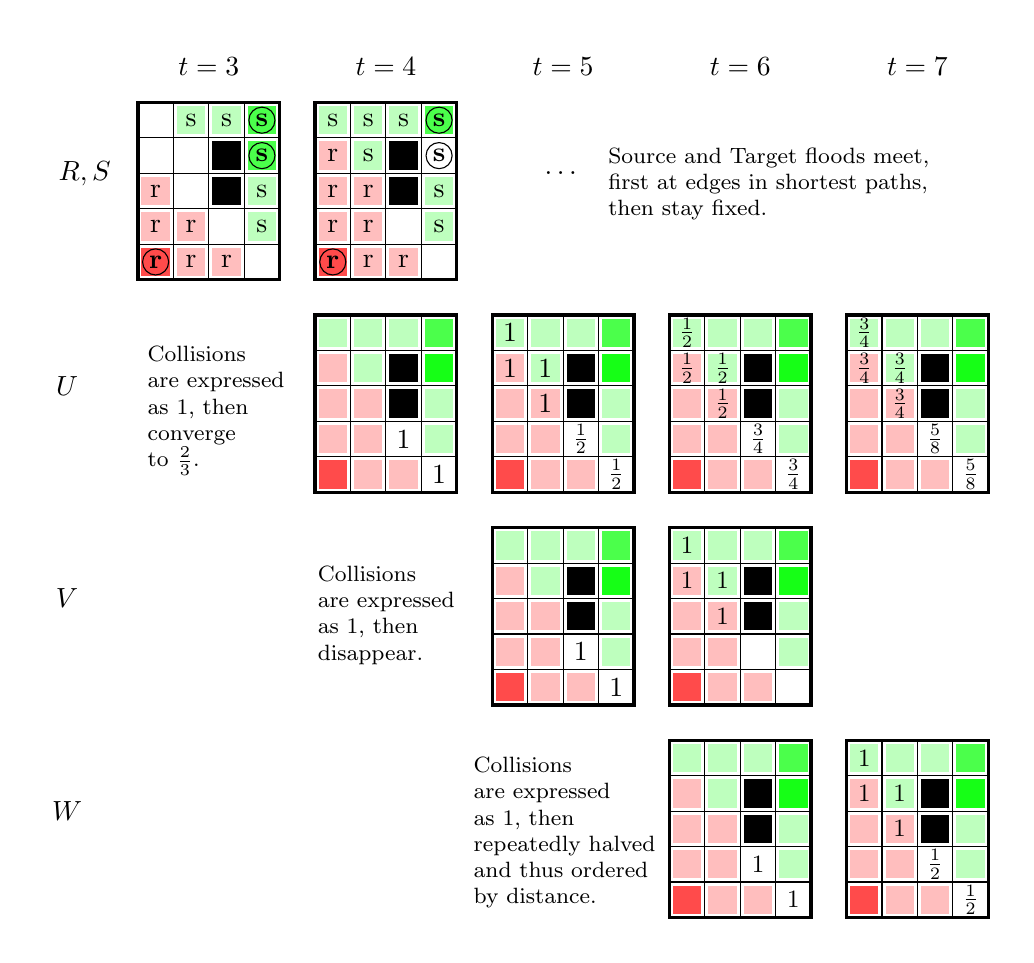
\begin{tikzpicture}[scale=.9,every node/.style={minimum size=1cm},on grid]
		
    %slanting: production of a set of n 'laminae' to be piled up. N=number of grids.
   %\begin{scope}[
   %        yshift=-83,every node/.append style={
   %        yslant=0.5,xslant=-1},yslant=0.5,xslant=-1
   %        ]
   %    % opacity to prevent graphical interference
   %    \fill[white,fill opacity=0.9] (0,0) rectangle (5,5);
   %    \draw[step=4mm, black] (0,0) grid (5,5); %defining grids
   %    \draw[step=1mm, red!50,thin] (3,1) grid (4,2);  %Nested Grid
   %    \draw[black,very thick] (0,0) rectangle (5,5);%marking borders
   %    \fill[red] (0.05,0.05) rectangle (0.35,0.35);
   %    %Idem as above, for the n-th grid:
   %\end{scope}
	\node[] at (-0.75cm, 1.5cm) {$R , S$};	
	\node[] at (-1cm, -1.5cm) {$U$};	
	\node[] at (-1cm, -4.5cm) {$V$};	
	\node[] at (-1cm, -7.5cm) {$W$};	
	\node[] at (6cm, 1.5cm) {\dots};	
	\node[] at (1, 3){$t=3$};
    \begin{scope}[
    	yshift=0,every node/.append style={
    	    },    	             ]
									 \fill[white,fill opacity=.9] (0,0) rectangle (2,2.5);
									 \draw[black,very thick] (0,0) rectangle (2,2.5);
									 \draw[step=5mm, black] (0,0) grid (2,2.5);
				\fill[red, opacity=0.7] (0.05, 0.05) rectangle ( .45, 0.45);
				\fill[black] (1.05, 1.55) rectangle (1.45, 1.95);
				\fill[black] (1.05, 1.05) rectangle (1.45, 1.45);
				\fill[green, opacity=0.7] (1.55, 2.05) rectangle (1.95, 2.45);
				\node[circle, draw, minimum size = 1] at (0.25, 0.25) {} ;
				\fill[red, opacity=0.25] (0.55, 0.05) rectangle ( .95, 0.45);
				\fill[red, opacity=0.25] (1.05, 0.05) rectangle ( 1.45, 0.45);
				\fill[red, opacity=0.25] (0.55, 0.55) rectangle ( .95, 0.95);
				\fill[red, opacity=0.25] (0.05, 0.55) rectangle ( .45, 0.95);
				\fill[red, opacity=0.25] (0.05, 1.05) rectangle ( .45, 1.45);
				\node[] at (0.25, 0.25) {\bf{r}};
				\node[] at (0.75, 0.75) {r};
				\node[] at (0.75, 0.25) {r};
				\node[] at (0.25, 0.75) {r};
				\node[] at (1.25, 0.25) {r};
				\node[] at (0.25, 1.25) {r};

				\node[circle, draw, minimum size = 1] at (1.75, 2.25) {} ;
				\fill[green, opacity=0.25] (1.05, 2.05) rectangle (1.45, 2.45);
				\fill[green, opacity=0.7] (1.55, 1.55) rectangle (1.95, 1.95);
				\fill[green, opacity=0.25] (1.55, 1.05) rectangle (1.95, 1.45);
				\fill[green, opacity=0.25] (1.55, 0.55) rectangle (1.95, 0.95);
				\fill[green, opacity=0.25] (0.55, 2.05) rectangle (0.95, 2.45);
				\node[circle, draw, minimum size = 1] at (1.75, 1.75) {} ;
				\node[] at (1.75, 2.25) {\bf{s}};
				\node[] at (1.75, 1.75) {\bf{s}};
				\node[] at (1.25, 2.25) {s};
				\node[] at (0.75, 2.25) {s};
				\node[] at (1.75, 1.25) {s};
				\node[] at (1.75, 0.75) {s};
    \end{scope}    	

		\node[] at (3.5, 3){$t=4$};
		\node[] at (6, 3){$t=5$};
		\node[] at (8.5, 3){$t=6$};
		\node[] at (11, 3){$t=7$};
    \begin{scope}[
				yshift=0, xshift=2.5cm,every node/.append style={
    	    },
    	             ]
									 \fill[white,fill opacity=.9] (0,0) rectangle (2,2.5);
									 \draw[black,very thick] (0,0) rectangle (2,2.5);
									 \draw[step=5mm, black] (0,0) grid (2,2.5);
				\fill[red, opacity=0.7] (0.05, 0.05) rectangle ( .45, 0.45);
				\fill[black] (1.05, 1.55) rectangle (1.45, 1.95);
				\fill[black] (1.05, 1.05) rectangle (1.45, 1.45);
				\fill[green, opacity=0.7] (1.55, 2.05) rectangle (1.95, 2.45);
				\node[circle, draw, minimum size = 1] at (0.25, 0.25) {} ;
				\fill[red, opacity=0.25] (0.55, 0.05) rectangle ( .95, 0.45);
				\fill[red, opacity=0.25] (1.05, 0.05) rectangle ( 1.45, 0.45);
				\fill[red, opacity=0.25] (0.55, 0.55) rectangle ( .95, 0.95);
				\fill[red, opacity=0.25] (0.05, 0.55) rectangle ( .45, 0.95);
				\fill[red, opacity=0.25] (0.05, 1.05) rectangle ( .45, 1.45);
				\fill[red, opacity=0.25] (0.05, 1.55) rectangle ( .45, 1.95);
				\fill[red, opacity=0.25] (0.55, 1.05) rectangle ( .95, 1.45);
				\node[] at (0.25, 0.25) {\bf{r}};
				\node[] at (0.75, 0.75) {r};
				\node[] at (0.75, 1.25) {r};
				\node[] at (0.75, 0.25) {r};
				\node[] at (0.25, 0.75) {r};
				\node[] at (1.25, 0.25) {r};
				\node[] at (0.25, 1.25) {r};
				\node[] at (0.25, 1.75) {r};

				\node[circle, draw, minimum size = 1] at (1.75, 2.25) {} ;
				\fill[green, opacity=0.25] (1.05, 2.05) rectangle (1.45, 2.45);
				\fill[green, opacity=0.25] (1.55, 1.05) rectangle (1.95, 1.45);
				\fill[green, opacity=0.25] (1.55, 0.55) rectangle (1.95, 0.95);
				\fill[green, opacity=0.25] (0.55, 2.05) rectangle (0.95, 2.45);
				\fill[green, opacity=0.25] (0.05, 2.05) rectangle (0.45, 2.45);
				\fill[green, opacity=0.25] (0.55, 1.55) rectangle (0.95, 1.95);
				\node[circle, draw, minimum size = 1] at (1.75, 1.75) {} ;
				\node[] at (1.75, 2.25) {\bf{s}};
				\node[] at (1.75, 1.75) {\bf{s}};
				\node[] at (1.25, 2.25) {s};
				\node[] at (0.75, 2.25) {s};
				\node[] at (0.75, 1.75) {s};
				\node[] at (0.25, 2.25) {s};
				\node[] at (1.75, 1.25) {s};
				\node[] at (1.75, 0.75) {s};
    \end{scope}

		
		\begin{scope}[
				yshift=-3cm, xshift=2.5cm,every node/.append style={
    	    },    	             ]
									 \fill[white,fill opacity=.9] (0,0) rectangle (2,2.5);
									 \draw[black,very thick] (0,0) rectangle (2,2.5);
									 \draw[step=5mm, black] (0,0) grid (2,2.5);
				\fill[red, opacity=0.7] (0.05, 0.05) rectangle ( .45, 0.45);
				\fill[red, opacity=0.25] (0.55, 0.05) rectangle ( .95, 0.45);
				\fill[red, opacity=0.25] (1.05, 0.05) rectangle ( 1.45, 0.45);
				\fill[red, opacity=0.25] (0.55, 0.55) rectangle ( .95, 0.95);
				\fill[red, opacity=0.25] (0.05, 0.55) rectangle ( .45, 0.95);
				\fill[red, opacity=0.25] (0.05, 1.05) rectangle ( .45, 1.45);
				\fill[red, opacity=0.25] (0.05, 1.55) rectangle ( .45, 1.95);
				\fill[red, opacity=0.25] (0.55, 1.05) rectangle ( .95, 1.45);
				\fill[black] (1.05, 1.55) rectangle (1.45, 1.95);
				\fill[black] (1.05, 1.05) rectangle (1.45, 1.45);
				\fill[green, opacity=0.7] (1.55, 2.05) rectangle (1.95, 2.45);
				\fill[green, opacity=0.7] (1.55, 1.55) rectangle (1.95, 1.95);
				\fill[green, opacity=0.25] (1.05, 2.05) rectangle (1.45, 2.45);
				\fill[green, opacity=0.7] (1.55, 1.55) rectangle (1.95, 1.95);
				\fill[green, opacity=0.25] (1.55, 1.05) rectangle (1.95, 1.45);
				\fill[green, opacity=0.25] (1.55, 0.55) rectangle (1.95, 0.95);
				\fill[green, opacity=0.25] (0.55, 2.05) rectangle (0.95, 2.45);
				\fill[green, opacity=0.25] (0.05, 2.05) rectangle (0.45, 2.45);
				\fill[green, opacity=0.25] (0.55, 1.55) rectangle (0.95, 1.95);
				\node[] at (1.75, 0.25) {$1$};
				\node[] at (1.25, 0.75) {$1$};
    \end{scope}

    \begin{scope}[
				yshift=-3cm, xshift=5cm,every node/.append style={
				},    	             ]
									 \fill[white,fill opacity=.9] (0,0) rectangle (2,2.5);
									 \draw[black,very thick] (0,0) rectangle (2,2.5);
									 \draw[step=5mm, black] (0,0) grid (2,2.5);
				\fill[red, opacity=0.7] (0.05, 0.05) rectangle ( .45, 0.45);
				\fill[red, opacity=0.25] (0.55, 0.05) rectangle ( .95, 0.45);
				\fill[red, opacity=0.25] (1.05, 0.05) rectangle ( 1.45, 0.45);
				\fill[red, opacity=0.25] (0.55, 0.55) rectangle ( .95, 0.95);
				\fill[red, opacity=0.25] (0.05, 0.55) rectangle ( .45, 0.95);
				\fill[red, opacity=0.25] (0.05, 1.05) rectangle ( .45, 1.45);
				\fill[red, opacity=0.25] (0.05, 1.55) rectangle ( .45, 1.95);
				\fill[red, opacity=0.25] (0.55, 1.05) rectangle ( .95, 1.45);
				\fill[black] (1.05, 1.55) rectangle (1.45, 1.95);
				\fill[black] (1.05, 1.05) rectangle (1.45, 1.45);
				\fill[green, opacity=0.7] (1.55, 2.05) rectangle (1.95, 2.45);
				\fill[green, opacity=0.7] (1.55, 1.55) rectangle (1.95, 1.95);
				\fill[green, opacity=0.25] (1.05, 2.05) rectangle (1.45, 2.45);
				\fill[green, opacity=0.7] (1.55, 1.55) rectangle (1.95, 1.95);
				\fill[green, opacity=0.25] (1.55, 1.05) rectangle (1.95, 1.45);
				\fill[green, opacity=0.25] (1.55, 0.55) rectangle (1.95, 0.95);
				\fill[green, opacity=0.25] (0.55, 2.05) rectangle (0.95, 2.45);
				\fill[green, opacity=0.25] (0.05, 2.05) rectangle (0.45, 2.45);
				\fill[green, opacity=0.25] (0.55, 1.55) rectangle (0.95, 1.95);
				\node[scale=0.9] at (1.75, 0.25) {$\frac{1}{2}$};
				\node[scale=0.9] at (1.25, 0.75) {$\frac{1}{2}$};
				\node[scale=1] at (0.25, 1.75) {$1$};
				\node[scale=1] at (0.25, 2.25) {$1$};
				\node[scale=1] at (0.75, 1.25) {$1$};
				\node[scale=1] at (0.75, 1.75) {$1$};
    \end{scope}

    \begin{scope}[
				yshift=-3cm, xshift=7.5cm,every node/.append style={
				},    	             ]
									 \fill[white,fill opacity=.9] (0,0) rectangle (2,2.5);
									 \draw[black,very thick] (0,0) rectangle (2,2.5);
									 \draw[step=5mm, black] (0,0) grid (2,2.5);
				\fill[red, opacity=0.7] (0.05, 0.05) rectangle ( .45, 0.45);
				\fill[red, opacity=0.25] (0.55, 0.05) rectangle ( .95, 0.45);
				\fill[red, opacity=0.25] (1.05, 0.05) rectangle ( 1.45, 0.45);
				\fill[red, opacity=0.25] (0.55, 0.55) rectangle ( .95, 0.95);
				\fill[red, opacity=0.25] (0.05, 0.55) rectangle ( .45, 0.95);
				\fill[red, opacity=0.25] (0.05, 1.05) rectangle ( .45, 1.45);
				\fill[red, opacity=0.25] (0.05, 1.55) rectangle ( .45, 1.95);
				\fill[red, opacity=0.25] (0.55, 1.05) rectangle ( .95, 1.45);
				\fill[black] (1.05, 1.55) rectangle (1.45, 1.95);
				\fill[black] (1.05, 1.05) rectangle (1.45, 1.45);
				\fill[green, opacity=0.7] (1.55, 2.05) rectangle (1.95, 2.45);
				\fill[green, opacity=0.7] (1.55, 1.55) rectangle (1.95, 1.95);
				\fill[green, opacity=0.25] (1.05, 2.05) rectangle (1.45, 2.45);
				\fill[green, opacity=0.7] (1.55, 1.55) rectangle (1.95, 1.95);
				\fill[green, opacity=0.25] (1.55, 1.05) rectangle (1.95, 1.45);
				\fill[green, opacity=0.25] (1.55, 0.55) rectangle (1.95, 0.95);
				\fill[green, opacity=0.25] (0.55, 2.05) rectangle (0.95, 2.45);
				\fill[green, opacity=0.25] (0.05, 2.05) rectangle (0.45, 2.45);
				\fill[green, opacity=0.25] (0.55, 1.55) rectangle (0.95, 1.95);
				\node[scale=0.9] at (1.75, 0.25) {$\frac{3}{4}$};
				\node[scale=0.9] at (1.25, 0.75) {$\frac{3}{4}$};
				\node[scale=0.9] at (0.25, 1.75) {$\frac{1}{2}$};
				\node[scale=0.9] at (0.25, 2.25) {$\frac{1}{2}$};
				\node[scale=0.9] at (0.75, 1.25) {$\frac{1}{2}$};
				\node[scale=0.9] at (0.75, 1.75) {$\frac{1}{2}$};
    \end{scope}

    \begin{scope}[
				yshift=-3cm, xshift=10cm,every node/.append style={
				},    	             ]
									 \fill[white,fill opacity=.9] (0,0) rectangle (2,2.5);
									 \draw[black,very thick] (0,0) rectangle (2,2.5);
									 \draw[step=5mm, black] (0,0) grid (2,2.5);
				\fill[red, opacity=0.7] (0.05, 0.05) rectangle ( .45, 0.45);
				\fill[red, opacity=0.25] (0.55, 0.05) rectangle ( .95, 0.45);
				\fill[red, opacity=0.25] (1.05, 0.05) rectangle ( 1.45, 0.45);
				\fill[red, opacity=0.25] (0.55, 0.55) rectangle ( .95, 0.95);
				\fill[red, opacity=0.25] (0.05, 0.55) rectangle ( .45, 0.95);
				\fill[red, opacity=0.25] (0.05, 1.05) rectangle ( .45, 1.45);
				\fill[red, opacity=0.25] (0.05, 1.55) rectangle ( .45, 1.95);
				\fill[red, opacity=0.25] (0.55, 1.05) rectangle ( .95, 1.45);
				\fill[black] (1.05, 1.55) rectangle (1.45, 1.95);
				\fill[black] (1.05, 1.05) rectangle (1.45, 1.45);
				\fill[green, opacity=0.7] (1.55, 2.05) rectangle (1.95, 2.45);
				\fill[green, opacity=0.7] (1.55, 1.55) rectangle (1.95, 1.95);
				\fill[green, opacity=0.25] (1.05, 2.05) rectangle (1.45, 2.45);
				\fill[green, opacity=0.7] (1.55, 1.55) rectangle (1.95, 1.95);
				\fill[green, opacity=0.25] (1.55, 1.05) rectangle (1.95, 1.45);
				\fill[green, opacity=0.25] (1.55, 0.55) rectangle (1.95, 0.95);
				\fill[green, opacity=0.25] (0.55, 2.05) rectangle (0.95, 2.45);
				\fill[green, opacity=0.25] (0.05, 2.05) rectangle (0.45, 2.45);
				\fill[green, opacity=0.25] (0.55, 1.55) rectangle (0.95, 1.95);
				\node[scale=0.9] at (1.75, 0.25) {$\frac{5}{8}$};
				\node[scale=0.9] at (1.25, 0.75) {$\frac{5}{8}$};
				\node[scale=0.9] at (0.25, 1.75) {$\frac{3}{4}$};
				\node[scale=0.9] at (0.25, 2.25) {$\frac{3}{4}$};
				\node[scale=0.9] at (0.75, 1.25) {$\frac{3}{4}$};
				\node[scale=0.9] at (0.75, 1.75) {$\frac{3}{4}$};
    \end{scope}




    \begin{scope}[
				yshift=-6cm, xshift=5cm,every node/.append style={
				},    	             ]
									 \fill[white,fill opacity=.9] (0,0) rectangle (2,2.5);
									 \draw[black,very thick] (0,0) rectangle (2,2.5);
									 \draw[step=5mm, black] (0,0) grid (2,2.5);
				\fill[red, opacity=0.7] (0.05, 0.05) rectangle ( .45, 0.45);
				\fill[red, opacity=0.25] (0.55, 0.05) rectangle ( .95, 0.45);
				\fill[red, opacity=0.25] (1.05, 0.05) rectangle ( 1.45, 0.45);
				\fill[red, opacity=0.25] (0.55, 0.55) rectangle ( .95, 0.95);
				\fill[red, opacity=0.25] (0.05, 0.55) rectangle ( .45, 0.95);
				\fill[red, opacity=0.25] (0.05, 1.05) rectangle ( .45, 1.45);
				\fill[red, opacity=0.25] (0.05, 1.55) rectangle ( .45, 1.95);
				\fill[red, opacity=0.25] (0.55, 1.05) rectangle ( .95, 1.45);
				\fill[black] (1.05, 1.55) rectangle (1.45, 1.95);
				\fill[black] (1.05, 1.05) rectangle (1.45, 1.45);
				\fill[green, opacity=0.7] (1.55, 2.05) rectangle (1.95, 2.45);
				\fill[green, opacity=0.7] (1.55, 1.55) rectangle (1.95, 1.95);
				\fill[green, opacity=0.25] (1.05, 2.05) rectangle (1.45, 2.45);
				\fill[green, opacity=0.7] (1.55, 1.55) rectangle (1.95, 1.95);
				\fill[green, opacity=0.25] (1.55, 1.05) rectangle (1.95, 1.45);
				\fill[green, opacity=0.25] (1.55, 0.55) rectangle (1.95, 0.95);
				\fill[green, opacity=0.25] (0.55, 2.05) rectangle (0.95, 2.45);
				\fill[green, opacity=0.25] (0.05, 2.05) rectangle (0.45, 2.45);
				\fill[green, opacity=0.25] (0.55, 1.55) rectangle (0.95, 1.95);
				\node[scale=1] at (1.75, 0.25) {$1$};
				\node[scale=1] at (1.25, 0.75) {$1$};
    \end{scope}

    \begin{scope}[
				yshift=-6cm, xshift=7.5cm,every node/.append style={
				},    	             ]
									 \fill[white,fill opacity=.9] (0,0) rectangle (2,2.5);
									 \draw[black,very thick] (0,0) rectangle (2,2.5);
									 \draw[step=5mm, black] (0,0) grid (2,2.5);
				\fill[red, opacity=0.7] (0.05, 0.05) rectangle ( .45, 0.45);
				\fill[red, opacity=0.25] (0.55, 0.05) rectangle ( .95, 0.45);
				\fill[red, opacity=0.25] (1.05, 0.05) rectangle ( 1.45, 0.45);
				\fill[red, opacity=0.25] (0.55, 0.55) rectangle ( .95, 0.95);
				\fill[red, opacity=0.25] (0.05, 0.55) rectangle ( .45, 0.95);
				\fill[red, opacity=0.25] (0.05, 1.05) rectangle ( .45, 1.45);
				\fill[red, opacity=0.25] (0.05, 1.55) rectangle ( .45, 1.95);
				\fill[red, opacity=0.25] (0.55, 1.05) rectangle ( .95, 1.45);
				\fill[black] (1.05, 1.55) rectangle (1.45, 1.95);
				\fill[black] (1.05, 1.05) rectangle (1.45, 1.45);
				\fill[green, opacity=0.7] (1.55, 2.05) rectangle (1.95, 2.45);
				\fill[green, opacity=0.7] (1.55, 1.55) rectangle (1.95, 1.95);
				\fill[green, opacity=0.25] (1.05, 2.05) rectangle (1.45, 2.45);
				\fill[green, opacity=0.7] (1.55, 1.55) rectangle (1.95, 1.95);
				\fill[green, opacity=0.25] (1.55, 1.05) rectangle (1.95, 1.45);
				\fill[green, opacity=0.25] (1.55, 0.55) rectangle (1.95, 0.95);
				\fill[green, opacity=0.25] (0.55, 2.05) rectangle (0.95, 2.45);
				\fill[green, opacity=0.25] (0.05, 2.05) rectangle (0.45, 2.45);
				\fill[green, opacity=0.25] (0.55, 1.55) rectangle (0.95, 1.95);
				\node[scale=0.9] at (1.75, 0.25) {};
				\node[scale=0.9] at (0.25, 1.75) {$1$};
				\node[scale=0.9] at (0.25, 2.25) {$1$};
				\node[scale=0.9] at (0.75, 1.25) {$1$};
				\node[scale=0.9] at (0.75, 1.75) {$1$};
    \end{scope}


    \begin{scope}[
				yshift=-9cm, xshift=7.5cm,every node/.append style={
				},    	             ]
									 \fill[white,fill opacity=.9] (0,0) rectangle (2,2.5);
									 \draw[black,very thick] (0,0) rectangle (2,2.5);
									 \draw[step=5mm, black] (0,0) grid (2,2.5);
				\fill[red, opacity=0.7] (0.05, 0.05) rectangle ( .45, 0.45);
				\fill[red, opacity=0.25] (0.55, 0.05) rectangle ( .95, 0.45);
				\fill[red, opacity=0.25] (1.05, 0.05) rectangle ( 1.45, 0.45);
				\fill[red, opacity=0.25] (0.55, 0.55) rectangle ( .95, 0.95);
				\fill[red, opacity=0.25] (0.05, 0.55) rectangle ( .45, 0.95);
				\fill[red, opacity=0.25] (0.05, 1.05) rectangle ( .45, 1.45);
				\fill[red, opacity=0.25] (0.05, 1.55) rectangle ( .45, 1.95);
				\fill[red, opacity=0.25] (0.55, 1.05) rectangle ( .95, 1.45);
				\fill[black] (1.05, 1.55) rectangle (1.45, 1.95);
				\fill[black] (1.05, 1.05) rectangle (1.45, 1.45);
				\fill[green, opacity=0.7] (1.55, 2.05) rectangle (1.95, 2.45);
				\fill[green, opacity=0.7] (1.55, 1.55) rectangle (1.95, 1.95);
				\fill[green, opacity=0.25] (1.05, 2.05) rectangle (1.45, 2.45);
				\fill[green, opacity=0.7] (1.55, 1.55) rectangle (1.95, 1.95);
				\fill[green, opacity=0.25] (1.55, 1.05) rectangle (1.95, 1.45);
				\fill[green, opacity=0.25] (1.55, 0.55) rectangle (1.95, 0.95);
				\fill[green, opacity=0.25] (0.55, 2.05) rectangle (0.95, 2.45);
				\fill[green, opacity=0.25] (0.05, 2.05) rectangle (0.45, 2.45);
				\fill[green, opacity=0.25] (0.55, 1.55) rectangle (0.95, 1.95);
				\node[scale=0.9] at (1.75, 0.25) {$1$};
				\node[scale=0.9] at (1.25, 0.75) {$1$};
    \end{scope}

    \begin{scope}[
				yshift=-9cm, xshift=10cm,every node/.append style={
				},    	             ]
									 \fill[white,fill opacity=.9] (0,0) rectangle (2,2.5);
									 \draw[black,very thick] (0,0) rectangle (2,2.5);
									 \draw[step=5mm, black] (0,0) grid (2,2.5);
				\fill[red, opacity=0.7] (0.05, 0.05) rectangle ( .45, 0.45);
				\fill[red, opacity=0.25] (0.55, 0.05) rectangle ( .95, 0.45);
				\fill[red, opacity=0.25] (1.05, 0.05) rectangle ( 1.45, 0.45);
				\fill[red, opacity=0.25] (0.55, 0.55) rectangle ( .95, 0.95);
				\fill[red, opacity=0.25] (0.05, 0.55) rectangle ( .45, 0.95);
				\fill[red, opacity=0.25] (0.05, 1.05) rectangle ( .45, 1.45);
				\fill[red, opacity=0.25] (0.05, 1.55) rectangle ( .45, 1.95);
				\fill[red, opacity=0.25] (0.55, 1.05) rectangle ( .95, 1.45);
				\fill[black] (1.05, 1.55) rectangle (1.45, 1.95);
				\fill[black] (1.05, 1.05) rectangle (1.45, 1.45);
				\fill[green, opacity=0.7] (1.55, 2.05) rectangle (1.95, 2.45);
				\fill[green, opacity=0.7] (1.55, 1.55) rectangle (1.95, 1.95);
				\fill[green, opacity=0.25] (1.05, 2.05) rectangle (1.45, 2.45);
				\fill[green, opacity=0.7] (1.55, 1.55) rectangle (1.95, 1.95);
				\fill[green, opacity=0.25] (1.55, 1.05) rectangle (1.95, 1.45);
				\fill[green, opacity=0.25] (1.55, 0.55) rectangle (1.95, 0.95);
				\fill[green, opacity=0.25] (0.55, 2.05) rectangle (0.95, 2.45);
				\fill[green, opacity=0.25] (0.05, 2.05) rectangle (0.45, 2.45);
				\fill[green, opacity=0.25] (0.55, 1.55) rectangle (0.95, 1.95);
				\node[scale=0.9] at (0.25, 1.75) {$1$};
				\node[scale=0.9] at (0.25, 2.25) {$1$};
				\node[scale=0.9] at (0.75, 1.25) {$1$};
				\node[scale=0.9] at (0.75, 1.75) {$1$};
				\node[scale=0.9] at (1.75, 0.25) {$\frac{1}{2}$};
				\node[scale=0.9] at (1.25, 0.75) {$\frac{1}{2}$};
    \end{scope}

\tikzset{story/.style={font=\footnotesize, anchor=north west, align=left}}
\node[story] at (6.5, 2) {Source and Target floods meet,\\first at edges in shortest paths,\\
 then stay fixed.};

\node[story] at (0, -0.8) {Collisions \\are expressed\\as $1$, then\\converge\\to $\frac{2}{3}$.};
\node[story] at (2.4, -3.9) {Collisions \\are expressed\\as $1$, then\\disappear.};
\node[story] at (4.6, -6.6) {Collisions \\are expressed\\as $1$, then\\repeatedly halved\\and thus ordered\\by distance.};

\end{tikzpicture}
\caption{Various channels of our Neural CA unrolled across time. Unless indicated otherwise, all cells have activations of $0$. Empty and unchanging channel-maps are omitted.}
\label{fig:floods}
\end{figure}
\section{Spanning Trees with Cellular Automata}

\label{app:CA}

We take our notation from \cite{behring2001algorithm}.
Our automaton, before applying its ruleset, copies the board over to an array of the same spatial dimensions, with additional (all-$0$) channels.
This representation will remain unchanged by the CA, and includes binary channels $R'$, $S'$ and $O$, encoding the presence of sources, targets, and obstacles, respectively.
Assume as well that channels $R'$ and $S'$ are copied to new channels $R$ and $S$ during this embedding. The later two channels will produce floods of activation emanating from source and target cells, respectively. The (symmetric) transition rules for these channels are as follows:

\begin{align*}
r_i^{t + 1} = 
	\begin{cases}
		1 & \text{if } r_i^t = 1 %\vee r'_i =1 % Deal with this in embedding, for now
		\vee 
			( \exists x \in \eta_i | r_x = 1 \wedge \neg\exists x\in \eta_i | s_x = 1 \wedge o_i \neq 1) \\
		0 & \text{otherwise}
	\end{cases} \\
s_i^{t + 1} = 
	\begin{cases}
		1 & \text{if } s_i^t = 1 %\vee s'_i = 1 
		\vee 
			(\exists x \in \eta_i | s_x = 1 \wedge \neg\exists x\in \eta_i | r_x = 1\wedge o_i \neq 1) \\
		0 & \text{otherwise}
	\end{cases}
\end{align*}

where $r_i^t$, $s_i^t$ are the states of the the cell $i$ at timestep $t$ in channels $R$ and $S$, respectively, and $\eta_i$ is the Von-Neumann neighbourhood of the cell $i$.

These floods of unit-activation on either channel will not overlap spatially; rather meeting to form a boundary, along which cells are halfway between each of some source-target pair.

Thus we define channels $U$ and $V$, which together act as a gate, passing an activation at these boundary cells---as soon as their VN neighbourhood is occupied by activations from both floods---to $W$, which will proceed by halving the received activation repeatedly, in order to track the temporal order in which border-cells were discovered (and by extension, the lengths of the paths to which they belong). 

The transition rule for the in-gate $U$ is:
\begin{align*}
	u_i^{t+1} = 
\begin{cases}
	1 & \text{if } u_i^t = 0 \wedge \exists x, y \in \eta_i | s_x = 1 \wedge s_y = 1 \\
	1 - u_i / 2 & \text{if } u_i > 0\\
	0 & \text{otherwise}
\end{cases} \\
\end{align*}
For any $u_i$, when floods collide in the patch $\eta_i$, then $u_i = 1$. At all following ticks, $u_i \in [1/2, 3/4]$, oscillating, to eventually converge to $2/3$. 

The out-gate $V$ has binary activation, with cells active only after being equal to $1$ in $U$:

\begin{align*}
	v_i^{t+1} =
	\begin{cases}
		1 & \text{if } u_i^t = 1 \\
		0 & \text{otherwise }
	\end{cases}
	\end{align*}
	Activations in $V$ will thus appear at a node $i$ two ticks after the floods have entered the neighbourhood $\eta_i$.

The timekeeper-channel $W$ is characterized by the following rule:
\begin{align*}
 w_i^t{t+1} =
\begin{cases}
	1 & \text{if } \exists x \in \eta_i | u_i = 1 \\
	w_i^t/2 & \text{if } w_i^t > 0 \\
	0 & \text{otherwise}
\end{cases}
\end{align*}
. Once $W$ is non-empty, the location of its least non-zero activation can be selected as the site for an edge-build---this edge being guaranteed to belong to the shortest path from the existing spanning tree to an unconnected node (or previous agent build).





\newpage
\bibliographystyle{unsrt}
\bibliography{references}


%\bibliography{references_old}
\end{appendices}
\end{document}
